\chapter{Threads}
Normalmente, la maggior parte delle applicazioni che funzionano nei sistemi moderni, sono implementate come un processo separato che ha controllo di più \textbf{thread}.

\begin{figure}[!htb]
    \centering
    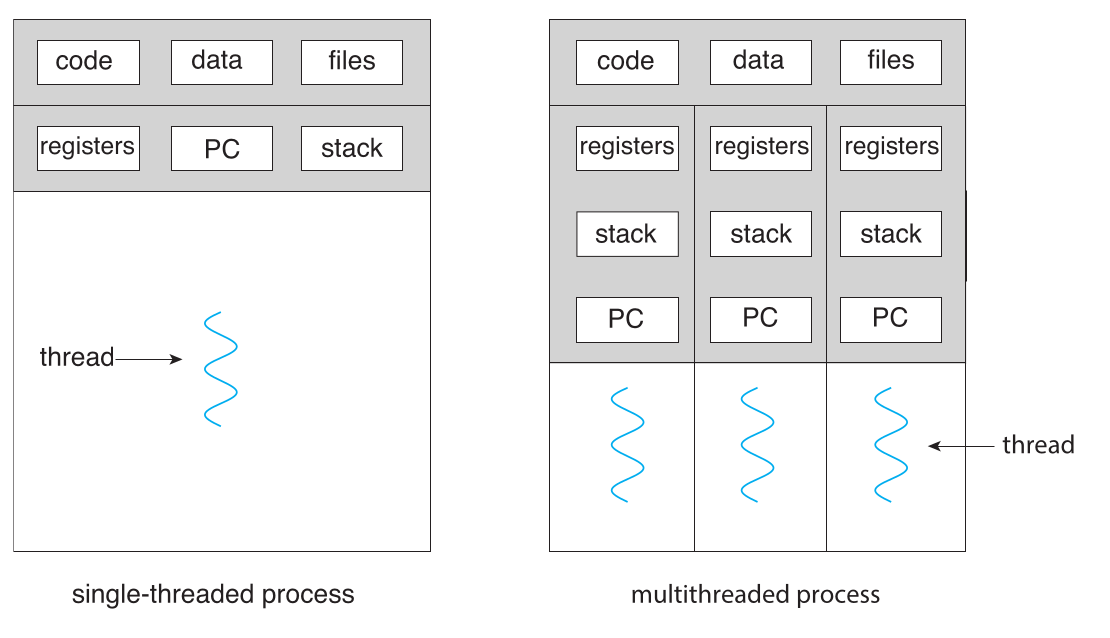
\includegraphics[width=0.5\linewidth]{Images/thread/ex.png}
    \caption{Singlethread VS Multithread.}
\end{figure}

Le applicazioni, possono venire programmate pure per essere \textbf{multicore}. \\ 
Per esempio, un server web in ascolto, potrebbe creare un nuovo processo per ogni richiesta che riceve, ma se a loro volta i processi ne creano altri, si potrebbe avere un overhead molto elevato.
Una soluzione è creare un thread che si mette in ascolto e, per ogni richiesta, crearne uno nuovo.

\begin{figure}[!htb]
    \centering
    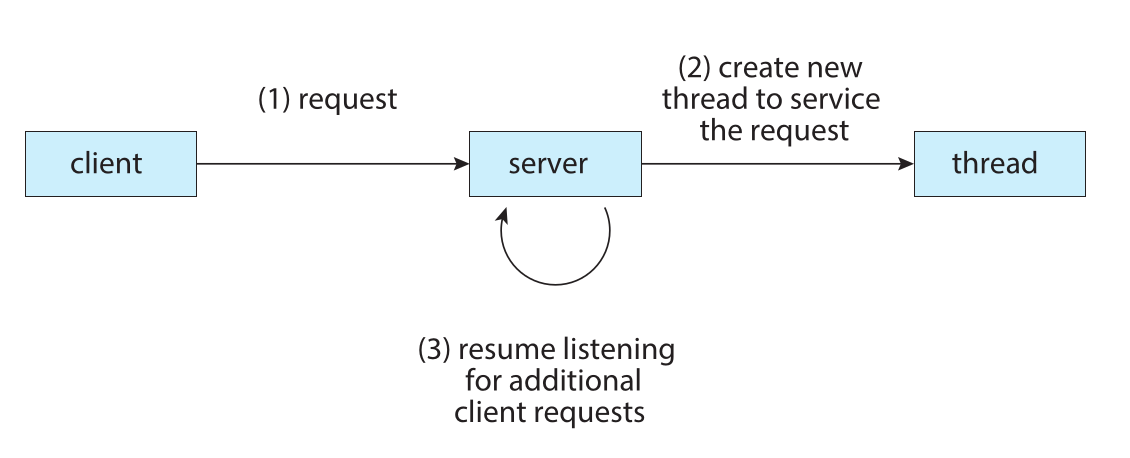
\includegraphics[width=0.6\linewidth]{Images/thread/server.png}
    \caption{Esempio di Utilizzo di Thread.}
\end{figure}

Utilizzare i thread garantisce molti benefici:
\begin{itemize}
  \item \textbf{Reattività:} permette di fare operazioni, anche se una parte di un processo è ferma. Molto utile per le interfacce grafiche.
  \item \textbf{Condivisione delle Risorse:} i processi necessitano di tecniche particolari per condividere le risorse, i thread, invece, condividono la memoria con il processi che li ha creati.
  \item \textbf{Economia:} creare nuovi thread e cambiare il contesto fra di loro occupa meno tempo e meno memoria. L'overhead introdotto è minore.
  \item \textbf{Scalabilità:} può trarre benficio molto dalla architetture multicore, eseguendo più thread contemporaneamente su più core.
\end{itemize}

\section{Programmazione Multicore}
I sistemi multicore consistono nell'inserire molteplici \textbf{core} di calcolo in un unico chip di elaborazione, 
in cui ciascun core appare al sistema operativo come una CPU distinta. La programmazione multithread offre un meccanismo per un utilizzo più efficiente di questi core di calcolo,
consentendo una maggiore concorrenza. \\
\vspace*{0.01\textheight}
In un sistema singlecore, avere più thread permette di avere \textbf{concorrenza}, invece, in un sistema multicore, permette di ottenere il \textbf{parallellismo}.

\begin{note}[NOTA BENE]
\textbf{Concorrenza $\ne$ Parallellismo }\\ 
Un sistema concorrente supporta più di un'attività, consentendo a tutte le attività di avanzare.
Al contrario, un sistema parallelo è in grado di eseguire più di un'attività simultaneamente.
\end{note}

\begin{defn}[Legge di Amdahl]
La legge di Amdahl è una formula che individua i potenziali incrementi di prestazioni derivanti dall'aggiunta di ulteriori core a un'applicazione che presenta sia componenti sequenziali che paralleli. 
\[
  \text{speedup} \le \frac{1}{S + \frac{(1-S)}{N}}
\]
Dove $S$ rappresenta la parte di calcolo sequenziale e $N$ il numero di core.
\end{defn}

\subsection{Tipi di Parallelismo}
Generalmente ci sono due tipi di parallellismo:
\begin{enumerate}
  \item \textbf{Parallelismo dei Dati:} cerca di dividere un insieme di dati in più sottoinsiemi e distribuirli su più core.
  \item \textbf{Parallelismo dei Task:} distribuire i thread sui core, ognuno eseguirà un suo task.
\end{enumerate}

\begin{figure}[!htb]
    \centering
    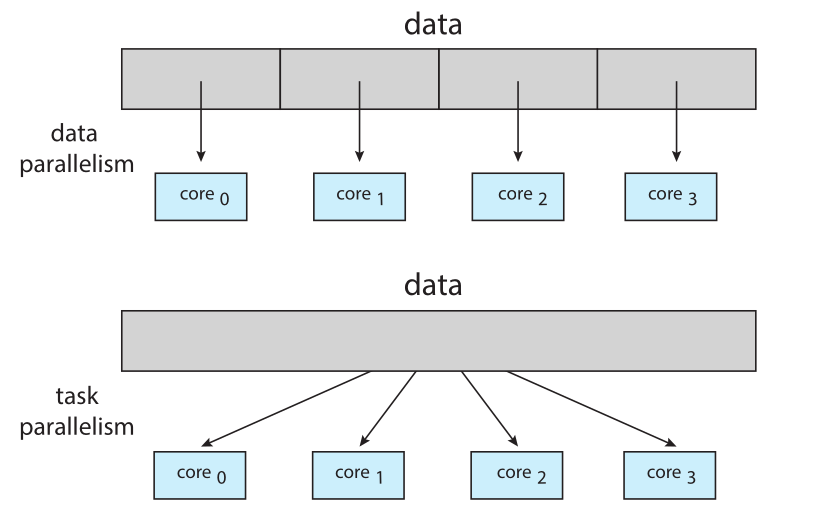
\includegraphics[width=0.6\linewidth]{Images/thread/parallelism.png}
    \caption{Tipi di Parallelismo.}
\end{figure}

\section{Modelli di Multithreading}
Esistono due tipi di thread:
\begin{enumerate}
  \item \textbf{User Thread:} gestiti da librerie nel livello utente (\texttt{pthread}, Windows Thread e Java Thread).
  \item \textbf{Kernel Thread:} supoortati del kernel di tutti i maggiori sistemi operativi.
\end{enumerate}

Inoltre, esistono tre modelli diversi per mappare i thread:
\begin{enumerate}
  \item \textbf{Many-To-One:} più thread user-level vengono mappati a un singolo kernel thread.
  \item \textbf{One-To-One:} ogni thread user-level viene mappato a un kernel thread.
  \item \textbf{Many-To-Many:} più thread user-level possono essere mappati su più kernel thread.
\end{enumerate}

\begin{figure}[!htb]
    \centering
    \begin{subfigure}{0.40\linewidth}
        \centering
        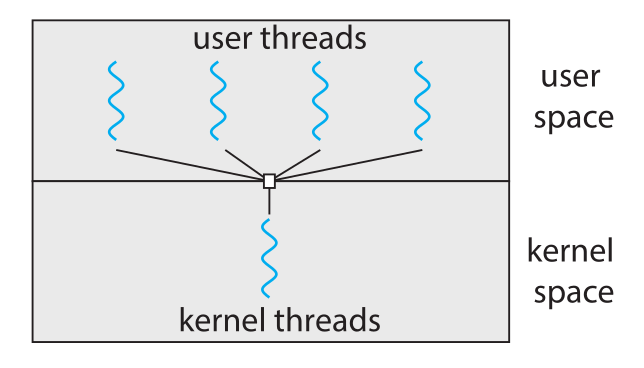
\includegraphics[width=\linewidth]{Images/thread/many-to-one.png}
        \caption{Modello Many-To-One.}
    \end{subfigure}
    \hfill
    \begin{subfigure}{0.40\linewidth}
        \centering
        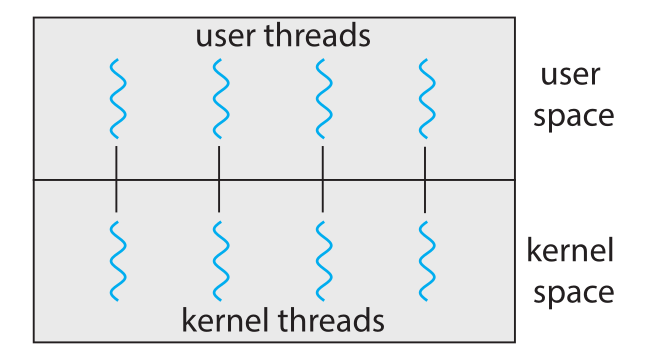
\includegraphics[width=\linewidth]{Images/thread/one-to-one.png}
        \caption{Modello One-To-One.}
    \end{subfigure}

     \begin{subfigure}{0.40\linewidth}
        \centering
        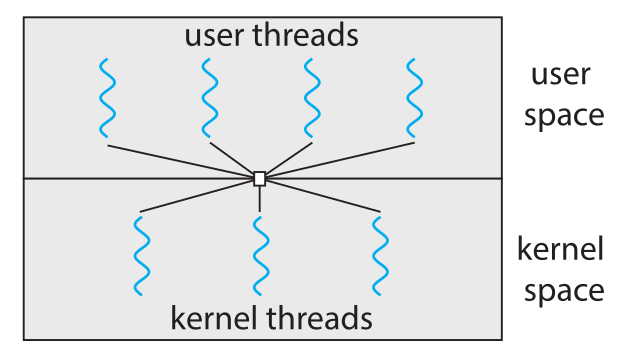
\includegraphics[width=\linewidth]{Images/thread/many-to-many.png}
        \caption{Modello Many-To-Many.}
    \end{subfigure}
\end{figure}



